\documentclass[12pt]{article}
\usepackage{amsmath}
\usepackage{amssymb}
\usepackage[letterpaper,top=1.35in,bottom=0.75in,left=0.75in,right=0.75in,centering]{geometry}
\usepackage{fancyhdr}
\usepackage{enumerate}
\usepackage{lastpage}
\usepackage{multicol}
\usepackage{graphicx}
\usepackage{vwcol}
\usepackage{tikz}
\usetikzlibrary{calc, positioning, decorations.pathmorphing}

\reversemarginpar

\pagestyle{fancy}
\cfoot{Page \thepage \ of \pageref{LastPage}}\rfoot{{\bf Total Points: 100}}
\lhead{\hspace*{2.2in}\underline{MATH 1560 Final}}

\newcommand{\points}[1]{\marginpar{\hspace{24pt}[#1]}}
\newcommand{\skipline}{\vspace{12pt}}
\renewcommand{\headrulewidth}{0in}
\headheight 20pt

\newcommand{\di}{\displaystyle}
\newcommand{\abs}[1]{\lvert #1\rvert}
\newcommand{\R}{\mathbb{R}}
\newcommand{\C}{\mathbb{C}}
\renewcommand{\P}{\mathcal{P}}
\DeclareMathOperator{\nul}{null}
\DeclareMathOperator{\range}{range}
\DeclareMathOperator{\spn}{span}
\newcommand{\len}[1]{\lVert #1\rVert}
\newcommand{\Q}{\mathbb{Q}}
\newcommand{\N}{\mathbb{N}}
\renewcommand{\L}{\mathcal{L}}
\newcommand{\dotp}{\boldsymbol{\cdot}}
\newenvironment{amatrix}[1]{%
  \left[\begin{array}{@{}*{#1}{c}|c@{}}
}{%
  \end{array}\right]
}
\newcommand{\bam}{\begin{amatrix}}
\newcommand{\eam}{\end{amatrix}}
\newcommand{\bbm}{\begin{bmatrix}}
\newcommand{\ebm}{\end{bmatrix}}

\begin{document}


\author{Instructor: Sean Fitzpatrick}
\thispagestyle{plain}
\begin{center}
\emph{University of Lethbridge}\\
Department of Mathematics and Computer Science\\
15 December, 2017\\
{\bf MATH 1560 - Final Exam}\\
Examiner: Sean Fitzpatrick
\end{center}
%\skipline \skipline \skipline \noindent \skipline
%Last Name:\underline{\hspace{350pt}}\\
%\skipline
%First Name:\underline{\hspace{348pt}}\\
%\skipline
%Student Number:\underline{\hspace{322pt}}\\
%\skipline



\vspace{0.1in}

\vspace*{\fill}

\begin{quote}
Print your name and student number clearly in the space above. You may remove this cover page, and use the back for scrap paper. If you want any work on the back of this page to be graded, you must clearly indicate this on the page containing the corresponding question.

\medskip

Answer the questions in the space provided. Show all work and necessary justification. Partial credit may be awarded for partially correct work.
 
\medskip

No outside aids are permitted, with the exception of a basic calculator. 
\end{quote}



\newpage

Extra space for rough work. And also, a unit circle.

\vspace*{\fill}

\begin{center}
 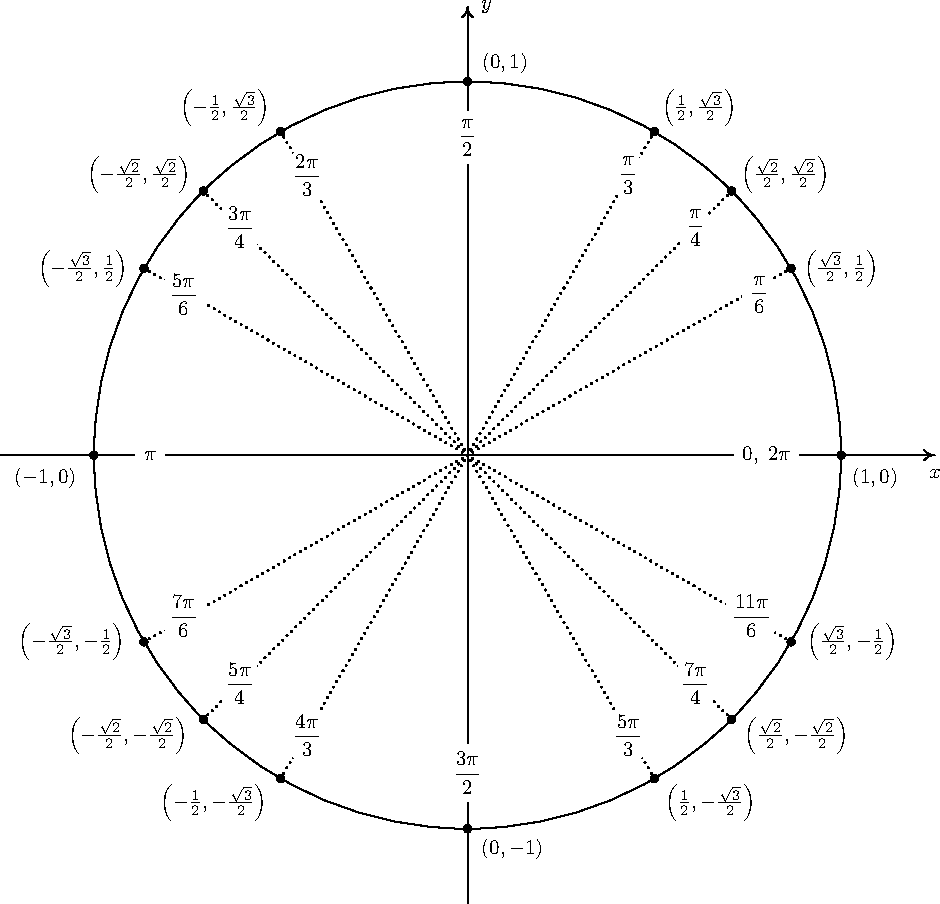
\includegraphics[scale=0.75]{UnitCircle}
\end{center}
\newpage

 \begin{enumerate}
 \item  Evaluate the following limits:
 \begin{enumerate}
 \item $\di \lim_{x\to 1}\frac{x^2+2x-3}{x^2-1}$ \points{2}
 
 \vspace{1.25in}
 
 \item $\di \lim_{x\to 9}\frac{x-9}{\sqrt{x}-3}$ \points{2}
 
 \vspace{1.25in}
 
 \item $\di \lim_{x\to 0}\frac{x}{\sin(3x)}$ \points{2}
 
 \vspace{1.5in}
 
 \item $\di \lim_{x\to 2^-}\frac{\abs{x-2}}{x-2}$ \points{2}
 
 \vspace{1.5in}
 
 \item $\di\lim_{x\to \infty}\frac{3x^2-x+2}{x^3+x+4}$ \points{2}
 \end{enumerate}
 \newpage
 
 \item Show that \points{5}
 \[
 f(x) = \begin{cases} 2x^2-5, & \text{ if } x\geq 2\\ x+1, & \text{ if } x<2\end{cases}
 \]
 is continuous at $x=2$.
 
 \vspace{3.25in}
 
 \item Using the \textbf{limit definition of the derivative}, find the slope of the tangent line to the graph $y=\dfrac{1}{x-2}$ at the point $(0,-1/2)$. \points{5}
 
 \newpage
 
 \item Compute the derivative $f'(x)$ for each of the following functions:
 \begin{enumerate}
 \item $f(x) = 2x^4-5x^3+3x-\sqrt{x}$. \points{2}
 
 \vspace{1.25in}
 
 \item $f(x) = \dfrac{1-x^5}{x^2}$. \points{2}
 
 \vspace{1.5in}
 
 \item $f(x) = x^3\ln(x)$ \points{2}
 
 \vspace{1.25in}
 
 \item $f(x) = \sin^3(x)+\sin(x^3)$ \points{2}
 
 \vspace{1.5in}
 
 \item $f(x) = \arcsin(e^x)$ \points{2}
 \end{enumerate}
 \newpage
 
 \item Using implicit differentiation, determine the equation of the tangent line to the curve \points{6}
 \[
 x^3y-3xy^2=x
 \]
 at the point $(2,1)$.
 
 \vspace{3.75in}
 
 \item Compute the derivative of \points{4}
 $f(x) = \ln\left(\dfrac{(2x+1)^6e^{4x}}{\sqrt{1+x^4}}\right)$ 
 
 

 \newpage
 
 \item Determine the absolute maximum and minimum values of $f(x) = x^3-3x$ on $[0,2]$. \points{4}
 
 \vspace{3.25in}
 
 \item Find all critical numbers of $f(x) = x(x-5)^{2/3}$, and classify each one as a local maximum, local minimum, or neither. \points{4}
 
 \vspace{3.25in}
 
 \item Give an example of a continuous function $f$ with a critical number $c$ such that $f'(c)$ does not exist. \points{2} 
 
 \newpage
 
 \item A function and its first and second derivatives are given by:
 \[
 f(x)=\frac{1}{9}x(x-4)^3,\quad f'(x) = \frac{4}{9}(x-1)(x-4)^2, \quad f''(x) = \frac{4}{3}(x-2)(x-4).
 \]
  
   
  \begin{enumerate}
  \item What is the domain of $f$? \points{1}
  
  \vspace{1cm}
  
  \item Give any intercepts or asymptotes in the graph of $f$. \points{1}
  
  \vspace{1cm}
  
  \item What are the critical points of $f$?  \points{1}
  
  \vspace{1.5cm}
  
  \item On what intervals is $f$ increasing/decreasing? \points{1}
  
  \vspace{2cm}
  
  \item What are the inflection points of $f$?  \points{1}
  
  \vspace{1.5cm}
  
  \item On what intervals is $f$ concave up/down? \points{1}
  
  \vspace{2cm}

   \item Sketch the graph of $f$. \points{4}
 
  \end{enumerate}
\newpage
 
  \item  A rectangular rabbit enclosure needs to be built with an area of 200 $\text{m}^2$. The enclosure is being built next to a crocodile compound, which is already fenced. \points{5} What is the minimum amount of fencing needed for the remaining three sides?
  
  \vspace{4in}
  
  \item The height of a triangle is increasing at a rate of 3 cm/min. At some point in time, the base of the \points{5} triangle is 12 cm long, and the height is 9 cm. At what rate must the base of the triangle be changing for the area to remain constant? 
  
  
  
  
  
  \newpage
  
  \item Use a linear approximation to estimate the value of $(1.2)^5$ \points{3}
  
  \vspace{2in}
  
  
  \item Calculate the following Taylor polynomials:
  \begin{enumerate}
  \item The degree 5 Maclaurin polynomial for $f(x)=\sin(x)$. \points{3}
  
  \vspace{2.75in}
  
  \item The degree 3 Taylor polynomial for $f(x) = \dfrac{1}{x^2}$ about $a=1$. \points{4}
  \end{enumerate}
  
  \newpage
  
  \item Compute the following indefinite integrals:
  \begin{enumerate}
  \item $\di \int \left(8x^3 - \frac{4}{x^2}+2\right)\,dx$ \points{2}
  
  \vspace{1.25in}
  
  \item $\di \int\left(\sec^2(x)+\frac{1}{x}\right)\,dx$ \points{2}
  \end{enumerate}
  
  \vspace{1.25in}
  
    \item Evaluate the following definite integrals:
  \begin{enumerate}
  \item $\di \int_0^2(x^2-2x)\,dx$ \points{3}
  
  \vspace{1.5in}
  
  \item $\di \int_0^{\sqrt{3}}\frac{x}{\sqrt{x^2+1}}\,dx$ \points{3}
  \end{enumerate}
  
  \newpage
  
  \item Use a Riemann sum with 4 rectangles and right endpoints to approximate the value of the integral $\di \int_0^2 (2x^2-x)\,dx$. \points{4}
  
  \vspace{3.25in}

\item Evaluate the indefinite integrals: 
  \begin{enumerate}
  \item $\di \int x\sin(x^2)\,dx$ \points{3}
  
  \vspace{2in}
  
  \item $\di \int \frac{x^3}{x^4+1}\,dx$ \points{3}
 
  \end{enumerate}  


\newpage

An extra problem for your entertainment and/or enlightenment, worth 5 bonus points.

\bigskip
\item Consider the function $\di F(x) = \int_1^x \frac{1}{t}\,dt$.
\begin{enumerate}
\item Confirm that $F(1)=0$ and $F'(x) = \dfrac{1}{x}$. (What well-known function satisfies these conditions?)

\vspace{0.75in}


\item Show that $\di \int_a^{ab} \frac{1}{t}\,dt = \int_1^b \frac{1}{t}\,dt$. (Hint: use the substitution $u=t/a$).

\vspace{1.75in}

\item Show that $F(ab)=F(a)+F(b)$ for $a,b>0$. \\
(Use the definition above, not properties of well-known functions like $\ln(x)$. You will need a property of definite integrals and your result from part (b).)

\vspace{1.5in}

\item Show that for $a>0$, $F(a^b) = bF(a)$. 
(Hint: try the substitution $u=t^{1/b}$, so $t=u^b$.)
\end{enumerate}
\end{enumerate}
\newpage

Extra space for rough work.
\end{document}